\documentclass[aspectratio=169]{beamer}
\usetheme{Madrid}
\usecolortheme{default}

\usepackage{amsmath, amssymb, amsthm}
\usepackage{tikz}
\usetikzlibrary{arrows.meta, positioning, calc}
\usepackage{algorithm2e}

\title{Flow Networks and the Max-Flow Min-Cut Theorem}
\author{}
\date{}

\newcommand{\R}{\mathbb{R}}

\begin{document}

% ============================================================
% TITLE
% ============================================================
\begin{frame}
  \titlepage
\end{frame}

% ============================================================
% OUTLINE
% ============================================================
\begin{frame}{Outline}
  \tableofcontents
\end{frame}

% ============================================================
% SECTION 1: MATCHINGS
% ============================================================
\section{Matchings and Alternating Paths}

\begin{frame}{Bipartite Graphs}
  \begin{definition}
    A \textbf{bipartite graph} is a graph $G = (V, E)$ whose vertex set can be
    partitioned into two disjoint sets $A$ and $B$ such that every edge connects
    a vertex in $A$ to a vertex in $B$.
  \end{definition}

  \vspace{1em}
  % TODO: Add a TikZ figure of a simple bipartite graph
  \begin{center}
    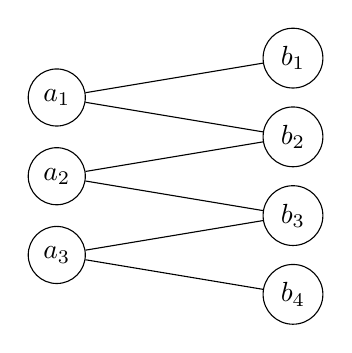
\begin{tikzpicture}[
      every node/.style={circle, draw, minimum size=6mm},
      >=Stealth
    ]
      \node (a1) at (0,2) {$a_1$};
      \node (a2) at (0,1) {$a_2$};
      \node (a3) at (0,0) {$a_3$};
      \node (b1) at (3,2.5) {$b_1$};
      \node (b2) at (3,1.5) {$b_2$};
      \node (b3) at (3,0.5) {$b_3$};
      \node (b4) at (3,-0.5) {$b_4$};
      \draw (a1) -- (b1);
      \draw (a1) -- (b2);
      \draw (a2) -- (b2);
      \draw (a2) -- (b3);
      \draw (a3) -- (b3);
      \draw (a3) -- (b4);
    \end{tikzpicture}
  \end{center}
\end{frame}

\begin{frame}{Matchings}
  \begin{definition}
    A \textbf{matching} $M$ in a graph $G = (V, E)$ is a set of pairwise
    non-adjacent edges, i.e., no two edges in $M$ share a common vertex.
  \end{definition}

  \begin{definition}
    A \textbf{maximum matching} is a matching of maximum cardinality.
    A \textbf{perfect matching} is a matching that saturates every vertex.
  \end{definition}

  \vspace{0.5em}
  % TODO: Add a TikZ figure highlighting a matching in a bipartite graph
\end{frame}

\begin{frame}{Alternating and Augmenting Paths}
  \begin{definition}
    Given a matching $M$, an \textbf{alternating path} is a path whose edges
    alternate between edges in $M$ and edges not in $M$.
  \end{definition}

  \begin{definition}
    An \textbf{augmenting path} is an alternating path that starts and ends at
    \textbf{unmatched} (free) vertices.
  \end{definition}

  \begin{theorem}[Berge's Theorem]
    A matching $M$ is maximum if and only if there is no augmenting path with
    respect to $M$.
  \end{theorem}
\end{frame}

\begin{frame}{Finding Maximum Matchings via Augmenting Paths}
  \textbf{Algorithm sketch:}
  \begin{enumerate}
    \item Start with an arbitrary matching $M$ (possibly empty).
    \item Search for an augmenting path $P$ with respect to $M$.
    \item If found, set $M \leftarrow M \oplus P$ (symmetric difference) to
          obtain a larger matching.
    \item Repeat until no augmenting path exists.
  \end{enumerate}

  \vspace{1em}
  % TODO: Add a step-by-step TikZ example of augmenting a matching
\end{frame}

% ============================================================
% SECTION 2: FROM MATCHINGS TO NETWORK FLOWS
% ============================================================
\section{From Matchings to Network Flows}

\begin{frame}{Adding a Source and Sink}
  Given a bipartite graph $G = (A \cup B, E)$:
  \begin{enumerate}
    \item Add a \textbf{source} $s$ with edges to every vertex in $A$.
    \item Add a \textbf{sink} $t$ with edges from every vertex in $B$.
    \item Direct all edges from $A$ to $B$.
    \item Set every edge capacity to $1$.
  \end{enumerate}

  \vspace{0.5em}
  \begin{center}
    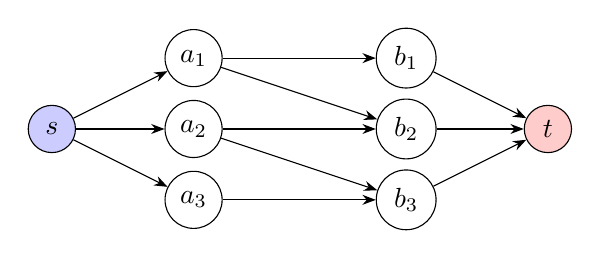
\begin{tikzpicture}[
      every node/.style={circle, draw, minimum size=6mm},
      >=Stealth, scale=0.9
    ]
      \node[fill=blue!20] (s) at (-2,1) {$s$};
      \node (a1) at (0,2) {$a_1$};
      \node (a2) at (0,1) {$a_2$};
      \node (a3) at (0,0) {$a_3$};
      \node (b1) at (3,2) {$b_1$};
      \node (b2) at (3,1) {$b_2$};
      \node (b3) at (3,0) {$b_3$};
      \node[fill=red!20] (t) at (5,1) {$t$};
      \draw[->] (s) -- (a1);
      \draw[->] (s) -- (a2);
      \draw[->] (s) -- (a3);
      \draw[->] (a1) -- (b1);
      \draw[->] (a1) -- (b2);
      \draw[->] (a2) -- (b2);
      \draw[->] (a2) -- (b3);
      \draw[->] (a3) -- (b3);
      \draw[->] (b1) -- (t);
      \draw[->] (b2) -- (t);
      \draw[->] (b3) -- (t);
    \end{tikzpicture}
  \end{center}

  A maximum matching in $G$ $\longleftrightarrow$ a maximum integer flow in this network.
\end{frame}

\begin{frame}{Why This Reduction Works}
  \begin{itemize}
    \item Unit capacities from $s$ ensure each $a_i$ is matched at most once.
    \item Unit capacities into $t$ ensure each $b_j$ is matched at most once.
    \item An integer flow of value $k$ corresponds to a matching of size $k$.
    \item Finding the \textbf{max flow} gives the \textbf{max matching}.
  \end{itemize}

  \vspace{1em}
  This motivates studying flows in general networks.
\end{frame}

\begin{frame}{Applications of Network Flow}
  \begin{itemize}
    \item \textbf{Bipartite matching:} Job assignments, course scheduling.
    \item \textbf{Transportation:} Shipping goods through a network at minimum cost.
    \item \textbf{Telecommunications:} Routing maximum data through a network.
    \item \textbf{Image segmentation:} Partitioning pixels via min-cut.
    \item \textbf{Baseball elimination:} Determining if a team can still win.
    \item \textbf{Airline scheduling:} Crew and aircraft assignment.
  \end{itemize}
\end{frame}

% ============================================================
% SECTION 3: FORMAL DEFINITIONS
% ============================================================
\section{Flows and Cuts: Formal Definitions}

\begin{frame}{Networks}
  \begin{definition}
    A \textbf{network} is a directed graph $G = (V, E)$ equipped with a
    non-negative \textbf{capacity function} $c : E \to \R_{\geq 0}$, and
    without multiple arcs.
  \end{definition}

  \vspace{0.5em}
  \textbf{Conventions:}
  \begin{itemize}
    \item If $(u,v) \in E$, we may assume $(v,u) \in E$ as well (possibly with
          $c(v,u) = 0$).
    \item If $(v,u) \notin E$, we add it with $c(v,u) = 0$.
  \end{itemize}
\end{frame}

\begin{frame}{Flow Networks}
  \begin{definition}
    A \textbf{flow network} is a tuple $(G, c, s, t)$ where:
    \begin{itemize}
      \item $G = (V, E)$ is a directed graph,
      \item $c : E \to \R_{\geq 0}$ is the capacity function,
      \item $s \in V$ is the \textbf{source},
      \item $t \in V$ is the \textbf{sink}, with $s \neq t$.
    \end{itemize}
  \end{definition}
\end{frame}

\begin{frame}{Flows}
  \begin{definition}
    A \textbf{flow} in $(G, c, s, t)$ is a function $f : E \to \R_{\geq 0}$
    satisfying:
    \begin{enumerate}
      \item \textbf{Capacity constraint:} $0 \leq f(u,v) \leq c(u,v)$ for all
            $(u,v) \in E$.
      \item \textbf{Conservation:} For every $v \in V \setminus \{s, t\}$,
            \[
              \sum_{u:(u,v)\in E} f(u,v) = \sum_{w:(v,w)\in E} f(v,w).
            \]
    \end{enumerate}
  \end{definition}

  \begin{definition}
    The \textbf{value} of a flow $f$ is
    \[
      |f| = \sum_{v:(s,v)\in E} f(s,v) - \sum_{u:(u,s)\in E} f(u,s).
    \]
  \end{definition}
\end{frame}

\begin{frame}{Cuts}
  \begin{definition}
    An \textbf{$s$-$t$ cut} is a partition $(S, T)$ of $V$ with $s \in S$ and
    $t \in T$.
  \end{definition}

  \begin{definition}
    The \textbf{capacity} of a cut $(S, T)$ is
    \[
      c(S, T) = \sum_{\substack{u \in S,\, v \in T \\ (u,v) \in E}} c(u,v).
    \]
  \end{definition}

  \vspace{0.5em}
  \textbf{Key observation:} For any flow $f$ and any $s$-$t$ cut $(S,T)$,
  \[
    |f| \leq c(S,T).
  \]
\end{frame}

% ============================================================
% SECTION 4: BEYOND BIPARTITE GRAPHS
% ============================================================
\section{Beyond Bipartite Graphs}

\begin{frame}{General Directed Graphs}
  The definitions of flow and cut apply to \textbf{any} directed graph --- not
  just bipartite ones.

  \vspace{1em}
  \textbf{Why bipartiteness doesn't matter:}
  \begin{itemize}
    \item Flow conservation is defined at every internal node regardless of
          graph structure.
    \item Capacity constraints are per-edge, independent of whether the graph
          is bipartite.
    \item The max-flow min-cut theorem holds for \emph{all} directed networks.
  \end{itemize}

  \vspace{1em}
  Bipartite matching was our \emph{motivation}, but the theory is fully general.
\end{frame}

\begin{frame}{Residual Graphs}
  \begin{definition}
    Given a flow $f$ in $(G, c, s, t)$, the \textbf{residual graph}
    $G_f = (V, E_f)$ has edges with \textbf{residual capacities}:
    \[
      c_f(u,v) =
      \begin{cases}
        c(u,v) - f(u,v) & \text{if } (u,v) \in E, \\
        f(v,u)           & \text{if } (v,u) \in E.
      \end{cases}
    \]
    An edge $(u,v) \in E_f$ if and only if $c_f(u,v) > 0$.
  \end{definition}

  \vspace{0.5em}
  An \textbf{augmenting path} in $G_f$ is any $s$-$t$ path in the residual
  graph.
\end{frame}

% ============================================================
% SECTION 5: MAX-FLOW MIN-CUT THEOREM
% ============================================================
\section{The Max-Flow Min-Cut Theorem}

\begin{frame}{Statement of the Theorem}
  \begin{theorem}[Max-Flow Min-Cut (Ford--Fulkerson, 1956)]
    In any flow network $(G, c, s, t)$, the following three conditions are
    equivalent:
    \begin{enumerate}
      \item $f$ is a maximum flow.
      \item There is no augmenting path in the residual graph $G_f$.
      \item There exists an $s$-$t$ cut $(S, T)$ such that $|f| = c(S, T)$.
    \end{enumerate}
  \end{theorem}

  \vspace{0.5em}
  Equivalently:
  \[
    \max_f |f| = \min_{(S,T)} c(S,T).
  \]
\end{frame}

\begin{frame}{Proof Sketch: (1) $\Rightarrow$ (2)}
  \textbf{Claim:} If $f$ is a maximum flow, then $G_f$ has no augmenting path.

  \vspace{1em}
  \textbf{Proof (contrapositive):}
  \begin{itemize}
    \item Suppose there exists an augmenting path $P$ in $G_f$.
    \item Let $\delta = \min_{(u,v) \in P} c_f(u,v) > 0$.
    \item Define $f'$ by pushing $\delta$ units along $P$:
          \[
            f'(u,v) =
            \begin{cases}
              f(u,v) + \delta & \text{forward edge on } P, \\
              f(u,v) - \delta & \text{backward edge on } P, \\
              f(u,v)          & \text{otherwise.}
            \end{cases}
          \]
    \item Then $|f'| = |f| + \delta > |f|$, so $f$ was not maximum. \qed
  \end{itemize}
\end{frame}

\begin{frame}{Proof Sketch: (2) $\Rightarrow$ (3)}
  \textbf{Claim:} If $G_f$ has no augmenting path, then there exists a cut
  $(S,T)$ with $|f| = c(S,T)$.

  \vspace{1em}
  \textbf{Proof:}
  \begin{itemize}
    \item Define $S = \{v \in V : v \text{ is reachable from } s \text{ in } G_f\}$.
    \item Set $T = V \setminus S$. Since there is no $s$-$t$ path in $G_f$, we
          have $t \in T$.
    \item For any $u \in S$, $v \in T$:
          \begin{itemize}
            \item $c_f(u,v) = 0$, so $f(u,v) = c(u,v)$ (edge saturated).
          \end{itemize}
    \item For any $u \in T$, $v \in S$:
          \begin{itemize}
            \item $f(u,v) = 0$ (otherwise $v$ would be reachable).
          \end{itemize}
    \item Therefore $|f| = c(S,T)$. \qed
  \end{itemize}
\end{frame}

\begin{frame}{Proof Sketch: (3) $\Rightarrow$ (1)}
  \textbf{Claim:} If $|f| = c(S,T)$ for some cut $(S,T)$, then $f$ is a
  maximum flow.

  \vspace{1em}
  \textbf{Proof:}
  \begin{itemize}
    \item For any flow $f'$ and any cut $(S', T')$, we have $|f'| \leq c(S',T')$.
    \item In particular, for our cut: $|f'| \leq c(S,T) = |f|$ for all flows $f'$.
    \item Hence $f$ is maximum. \qed
  \end{itemize}
\end{frame}

% ============================================================
% SECTION 6: FORD-FULKERSON ALGORITHM
% ============================================================
\section{The Ford--Fulkerson Algorithm}

\begin{frame}{Ford--Fulkerson Method}
  \begin{algorithm}[H]
    \SetAlgoLined
    \KwIn{Flow network $(G, c, s, t)$}
    \KwOut{Maximum flow $f$}
    Initialize $f(u,v) \leftarrow 0$ for all $(u,v) \in E$\;
    \While{there exists an augmenting path $P$ in $G_f$}{
      $\delta \leftarrow \min_{(u,v) \in P} c_f(u,v)$\;
      \ForEach{edge $(u,v) \in P$}{
        \eIf{$(u,v)$ is a forward edge}{
          $f(u,v) \leftarrow f(u,v) + \delta$\;
        }{
          $f(v,u) \leftarrow f(v,u) - \delta$\;
        }
      }
    }
    \Return{$f$}\;
  \end{algorithm}
\end{frame}

\begin{frame}{Edmonds--Karp: BFS Augmenting Paths}
  \begin{itemize}
    \item Ford--Fulkerson does not specify \emph{how} to find augmenting paths.
    \item With arbitrary paths and irrational capacities, it may not terminate.
    \item \textbf{Edmonds--Karp (1972):} Always choose a \textbf{shortest}
          augmenting path (via BFS).
    \item Guarantees $O(VE)$ augmentations $\Rightarrow$ $O(VE^2)$ total time.
  \end{itemize}
\end{frame}

\begin{frame}{Worked Example}
  % TODO: Replace with a concrete step-by-step flow example
  Consider the following network:

  \begin{center}
    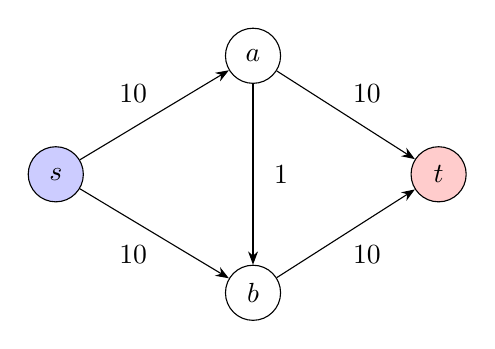
\begin{tikzpicture}[
      every node/.style={circle, draw, minimum size=7mm},
      >=Stealth, node distance=2cm
    ]
      \node[fill=blue!20] (s) {$s$};
      \node[above right=1cm and 2cm of s] (a) {$a$};
      \node[below right=1cm and 2cm of s] (b) {$b$};
      \node[fill=red!20, right=2cm of $(a)!0.5!(b)$] (t) {$t$};

      \draw[->] (s) -- node[above left, draw=none]{10} (a);
      \draw[->] (s) -- node[below left, draw=none]{10} (b);
      \draw[->] (a) -- node[right, draw=none]{1} (b);
      \draw[->] (a) -- node[above right, draw=none]{10} (t);
      \draw[->] (b) -- node[below right, draw=none]{10} (t);
    \end{tikzpicture}
  \end{center}

  \begin{itemize}
    \item \textbf{Step 1:} Find augmenting path $s \to a \to t$, push 10 units.
    \item \textbf{Step 2:} Find augmenting path $s \to b \to t$, push 10 units.
    \item \textbf{Step 3:} No augmenting path remains. Max flow $= 20$.
    \item \textbf{Min cut:} $S = \{s\}$, $T = \{a, b, t\}$, capacity $= 10 + 10 = 20$.
  \end{itemize}
\end{frame}

% ============================================================
% SECTION 7: SUMMARY AND RELATED THEOREMS
% ============================================================
\section{Summary and Related Theorems}

\begin{frame}{Hall's Marriage Theorem}
  \begin{theorem}[Hall, 1935]
    A bipartite graph $G = (A \cup B, E)$ has a matching that saturates every
    vertex in $A$ if and only if for every subset $S \subseteq A$,
    \[
      |N(S)| \geq |S|,
    \]
    where $N(S)$ is the set of neighbors of $S$ in $B$.
  \end{theorem}

  \vspace{0.5em}
  % TODO: Add proof sketch or note that it follows from max-flow min-cut
  This can be derived as a consequence of the max-flow min-cut theorem applied
  to the bipartite flow network.
\end{frame}

\begin{frame}{K\"{o}nig--Egerv\'{a}ry Theorem}
  \begin{theorem}[K\"{o}nig, 1931; Egerv\'{a}ry, 1931]
    In any bipartite graph, the size of a maximum matching equals the size of a
    minimum vertex cover.
  \end{theorem}

  \vspace{0.5em}
  \textbf{Connection to flows:}
  \begin{itemize}
    \item Maximum matching $\longleftrightarrow$ max flow in bipartite network.
    \item Minimum vertex cover $\longleftrightarrow$ min cut.
    \item K\"{o}nig--Egerv\'{a}ry is the max-flow min-cut theorem specialized
          to bipartite graphs with unit capacities.
  \end{itemize}
\end{frame}

\begin{frame}{Birkhoff--von Neumann Theorem}
  \begin{theorem}[Birkhoff, 1946; von Neumann, 1953]
    Every doubly stochastic matrix is a convex combination of permutation
    matrices.
  \end{theorem}

  \vspace{0.5em}
  \textbf{Connection:}
  \begin{itemize}
    \item A doubly stochastic matrix defines a fractional perfect matching on
          $K_{n,n}$.
    \item By the integrality of network flow, every fractional perfect matching
          in a bipartite graph is a convex combination of integral perfect
          matchings.
    \item Permutation matrices correspond to perfect matchings in $K_{n,n}$.
  \end{itemize}
\end{frame}

\begin{frame}{Menger's Theorem}
  \begin{theorem}[Menger, 1927]
    The maximum number of \textbf{edge-disjoint} $s$-$t$ paths equals the
    minimum number of edges whose removal disconnects $s$ from $t$.
  \end{theorem}

  \vspace{0.5em}
  \textbf{Connection:}
  \begin{itemize}
    \item Set all edge capacities to $1$.
    \item Max flow $=$ number of edge-disjoint paths (integrality).
    \item Min cut $=$ minimum number of edges separating $s$ from $t$.
    \item Menger's theorem \emph{is} the max-flow min-cut theorem with unit
          capacities.
  \end{itemize}

  \vspace{0.5em}
  A vertex-connectivity version also holds (split each vertex into two nodes).
\end{frame}

\begin{frame}{Summary}
  \begin{enumerate}
    \item \textbf{Matchings} in bipartite graphs are found via augmenting paths.
    \item Adding a source and sink transforms matching into a \textbf{network flow}
          problem.
    \item \textbf{Flows} and \textbf{cuts} are defined on general directed graphs.
    \item The \textbf{Max-Flow Min-Cut Theorem} unifies these ideas:
          $\max |f| = \min c(S,T)$.
    \item Classical theorems follow as corollaries:
          \begin{itemize}
            \item Hall's Marriage Theorem
            \item K\"{o}nig--Egerv\'{a}ry Theorem
            \item Birkhoff--von Neumann Theorem
            \item Menger's Theorem
          \end{itemize}
  \end{enumerate}
\end{frame}

\begin{frame}{}
  \centering
  \Huge Thank You \\[1em]
  \large Questions?
\end{frame}

\end{document}
